\documentclass[11pt,a4paper]{article}

\usepackage[margin=1in]{geometry}
\usepackage{mathptmx}
\usepackage{amsmath}
\usepackage{amssymb}
\usepackage{amsthm}
\usepackage{braket}
\usepackage{tikz}
\usepackage{quantikz}
\usepackage{enumitem}
\usepackage{hyperref}
\usepackage{xcolor}

\definecolor{circuitblue}{RGB}{40,80,160}

\hypersetup{
    colorlinks=true,
    linkcolor=circuitblue,
    urlcolor=circuitblue,
    citecolor=circuitblue
}

\theoremstyle{definition}
\newtheorem{definition}{Definition}[section]
\newtheorem{example}{Example}[section]

\theoremstyle{remark}
\newtheorem*{intuition}{Intuition}
\newtheorem*{keypoint}{Key Point}

\pagestyle{plain}

\setlength{\parindent}{0pt}
\setlength{\parskip}{6pt}

\begin{document}

\begin{center}
    {\LARGE \textbf{Introduction to Classical Machine Learning}}\\[8pt]
    {\large QML}\\[12pt]
    \hrule
\end{center}

\vspace{12pt}
\tableofcontents
\newpage

%% ========================================================
\section{Why Classical ML in a Quantum Course?}
%% ========================================================

before u can understand \textbf{quantum} machine learning, u need to understand \textbf{machine learning}. QML is not a replacement for classical ML --- its an extension. the same concepts (loss functions, optimization, generalization, bias-variance tradeoff) apply directly. if u dont know classical ML well, QML will just be confusing notation on top of confusion.

this lecture covers the classical ML foundations that the rest of the course builds on. everything here has a quantum analogue that well encounter in later lectures.

%% ========================================================
\section{The Machine Learning Landscape}
%% ========================================================

\subsection{Supervised Learning}

\begin{definition}
in \textbf{supervised learning}, u have a dataset of input-output pairs $\{(x_i, y_i)\}_{i=1}^N$ and want to learn a function $f: X \to Y$ that maps inputs to outputs. the goal is to generalize --- predict $y$ for new, unseen $x$.
\end{definition}

two main flavors:
\begin{itemize}
    \item \textbf{classification}: $y$ is discrete (a label). e.g., is this email spam or not? is this image a cat or dog?
    \item \textbf{regression}: $y$ is continuous. e.g., predict house prices, stock returns, temperature.
\end{itemize}

\begin{center}
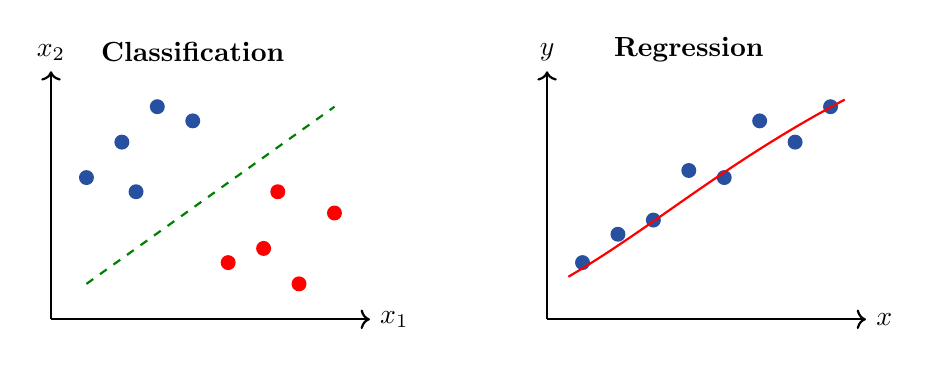
\begin{tikzpicture}[scale=0.9]
    % classification
    \begin{scope}
        \node[above, font=\bfseries] at (2,3.5) {Classification};
        \draw[->, thick] (0,0) -- (4.5,0) node[right] {$x_1$};
        \draw[->, thick] (0,0) -- (0,3.5) node[above] {$x_2$};
        % class 1 (blue)
        \fill[circuitblue] (1,2.5) circle (3pt);
        \fill[circuitblue] (1.5,3) circle (3pt);
        \fill[circuitblue] (0.5,2) circle (3pt);
        \fill[circuitblue] (2,2.8) circle (3pt);
        \fill[circuitblue] (1.2,1.8) circle (3pt);
        % class 2 (red)
        \fill[red] (3,1) circle (3pt);
        \fill[red] (3.5,0.5) circle (3pt);
        \fill[red] (2.5,0.8) circle (3pt);
        \fill[red] (4,1.5) circle (3pt);
        \fill[red] (3.2,1.8) circle (3pt);
        % decision boundary
        \draw[dashed, thick, green!50!black] (0.5,0.5) -- (4,3);
    \end{scope}

    % regression
    \begin{scope}[xshift=7cm]
        \node[above, font=\bfseries] at (2,3.5) {Regression};
        \draw[->, thick] (0,0) -- (4.5,0) node[right] {$x$};
        \draw[->, thick] (0,0) -- (0,3.5) node[above] {$y$};
        \fill[circuitblue] (0.5,0.8) circle (3pt);
        \fill[circuitblue] (1,1.2) circle (3pt);
        \fill[circuitblue] (1.5,1.4) circle (3pt);
        \fill[circuitblue] (2,2.1) circle (3pt);
        \fill[circuitblue] (2.5,2.0) circle (3pt);
        \fill[circuitblue] (3,2.8) circle (3pt);
        \fill[circuitblue] (3.5,2.5) circle (3pt);
        \fill[circuitblue] (4,3.0) circle (3pt);
        \draw[thick, red] (0.3,0.6) .. controls (1.5,1.3) and (2.5,2.2) .. (4.2,3.1);
    \end{scope}
\end{tikzpicture}
\end{center}

\subsection{Unsupervised Learning}

\begin{definition}
in \textbf{unsupervised learning}, u only have inputs $\{x_i\}$ --- no labels. the goal is to discover structure in the data.
\end{definition}

main tasks:
\begin{itemize}
    \item \textbf{clustering}: group similar data points together (e.g., k-means, DBSCAN)
    \item \textbf{dimensionality reduction}: find low-dimensional representations (e.g., PCA, t-SNE, autoencoders)
    \item \textbf{density estimation}: learn the probability distribution of the data (e.g., GMMs, normalizing flows)
    \item \textbf{generative modeling}: learn to generate new data that looks like the training data (e.g., GANs, VAEs)
\end{itemize}

\begin{keypoint}
for QML:
\begin{itemize}
    \item quantum classifiers (variational quantum classifiers, quantum kernel classifiers) $\to$ supervised classification
    \item quantum generative adversarial networks (QGANs) $\to$ generative modeling
    \item quantum kernel methods $\to$ both classification and regression
    \item quantum autoencoders $\to$ dimensionality reduction
    \item quantum boltzmann machines $\to$ density estimation / generative modeling
\end{itemize}
\end{keypoint}

\subsection{Reinforcement Learning (Brief)}

\begin{definition}
in \textbf{reinforcement learning} (RL), an agent interacts with an environment, taking actions and receiving rewards. the goal is to learn a policy that maximizes cumulative reward.
\end{definition}

RL is less directly connected to the QML methods covered in this course, but there is quantum RL research (using quantum circuits as policy networks, quantum advantage in certain RL settings). we wont go deep into it here.

%% ========================================================
\section{The Learning Framework}
%% ========================================================

\subsection{Hypothesis Class and Model}

\begin{definition}
a \textbf{hypothesis class} $\mathcal{H}$ is the set of all functions ur model can represent. a \textbf{model} with parameters $\theta$ defines a specific function $f_\theta \in \mathcal{H}$.
\end{definition}

\begin{example}
\begin{itemize}
    \item linear models: $\mathcal{H} = \{f(x) = w^T x + b\}$ --- all affine functions
    \item polynomial models: $\mathcal{H} = \{f(x) = \sum_{k=0}^d a_k x^k\}$ --- polynomials up to degree $d$
    \item neural networks: $\mathcal{H} = \{f_\theta(x)\}$ where $\theta$ r the weights and biases --- very large (often over-parameterized) hypothesis classes
    \item quantum models: $\mathcal{H} = \{\text{tr}(O \cdot U(\theta, x)\rho_0 U^\dagger(\theta, x))\}$ --- functions computed by parameterized quantum circuits
\end{itemize}
\end{example}

\subsection{Loss Functions}

\begin{definition}
a \textbf{loss function} $\mathcal{L}(f_\theta, x, y)$ measures how badly the model's prediction $f_\theta(x)$ disagrees with the true label $y$. the goal is to minimize the \textbf{empirical risk} (average loss over training data):
\[
\boxed{R_{\text{emp}}(\theta) = \frac{1}{N}\sum_{i=1}^N \mathcal{L}(f_\theta(x_i), y_i)}
\]
\end{definition}

common loss functions:

\textbf{mean squared error (MSE)} --- for regression:
\[
\mathcal{L}_{\text{MSE}} = \frac{1}{N}\sum_{i=1}^N (f_\theta(x_i) - y_i)^2
\]

\textbf{cross-entropy loss} --- for classification:
\[
\mathcal{L}_{\text{CE}} = -\frac{1}{N}\sum_{i=1}^N \left[y_i \log(p_i) + (1-y_i)\log(1-p_i)\right]
\]
where $p_i = f_\theta(x_i)$ is the predicted probability.

\textbf{hinge loss} --- for SVMs:
\[
\mathcal{L}_{\text{hinge}} = \frac{1}{N}\sum_{i=1}^N \max(0, 1 - y_i \cdot f_\theta(x_i))
\]
where $y_i \in \{-1, +1\}$.

\begin{intuition}
the choice of loss function encodes ur assumptions:
\begin{itemize}
    \item MSE assumes gaussian noise and penalizes large errors quadratically
    \item cross-entropy assumes bernoulli/categorical distributions and is well-calibrated for probabilities
    \item hinge loss only cares abt the margin (distance from the decision boundary) and ignores correctly classified points far from the boundary
\end{itemize}
in QML, loss functions r typically expectation values of observables: $\mathcal{L} = \langle O \rangle$ or functions thereof. the connection between classical and quantum loss functions is important for understanding variational algorithms.
\end{intuition}

%% ========================================================
\section{Bias-Variance Tradeoff}
%% ========================================================

\subsection{Decomposition}

the expected test error of a model can be decomposed as:
\[
\boxed{\text{expected error} = \text{bias}^2 + \text{variance} + \text{irreducible noise}}
\]

\begin{definition}
\begin{itemize}
    \item \textbf{bias}: error from wrong assumptions in the model. high bias $=$ underfitting --- the model is too simple to capture the true pattern.
    \item \textbf{variance}: error from sensitivity to training data fluctuations. high variance $=$ overfitting --- the model memorizes noise in the training data.
    \item \textbf{irreducible noise}: inherent randomness in the data that no model can capture.
\end{itemize}
\end{definition}

\begin{center}
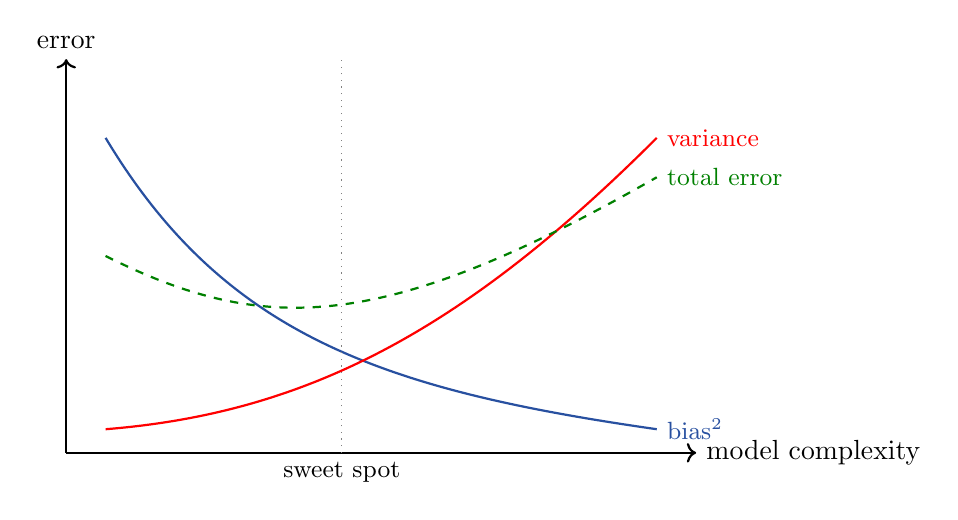
\begin{tikzpicture}[scale=1]
    \draw[->, thick] (0,0) -- (8,0) node[right] {model complexity};
    \draw[->, thick] (0,0) -- (0,5) node[above] {error};

    \draw[thick, circuitblue] (0.5,4) .. controls (2,1.5) and (4,0.8) .. (7.5,0.3) node[right, font=\small] {bias$^2$};
    \draw[thick, red] (0.5,0.3) .. controls (3,0.5) and (5,1.5) .. (7.5,4) node[right, font=\small] {variance};
    \draw[thick, green!50!black, dashed] (0.5,2.5) .. controls (2.5,1.5) and (4,1.5) .. (7.5,3.5) node[right, font=\small] {total error};

    \draw[dotted, gray] (3.5,0) -- (3.5,5);
    \node[below, font=\small] at (3.5,0) {sweet spot};
\end{tikzpicture}
\end{center}

\begin{keypoint}
for QML, the bias-variance tradeoff maps directly:
\begin{itemize}
    \item \textbf{circuit too shallow} (few parameters): high bias, underfitting. the quantum model cant express the target function.
    \item \textbf{circuit too deep} (many parameters): high variance, overfitting. the model fits noise. also noise from the hardware adds variance.
    \item \textbf{additional complication}: quantum noise adds a \textbf{third source of error} beyond classical bias and variance. this is unique to QML on NISQ hardware.
\end{itemize}
\end{keypoint}

%% ========================================================
\section{Overfitting and Regularization}
%% ========================================================

\subsection{Overfitting}

\begin{definition}
\textbf{overfitting} occurs when the model performs well on training data but poorly on test data. the model has learned the noise in the training set rather than the underlying pattern.
\end{definition}

\begin{example}
fitting a degree-20 polynomial to 10 data points: the polynomial passes through all training points perfectly (training error = 0) but oscillates wildly between points, giving terrible predictions on new data.
\end{example}

\subsection{Regularization Techniques}

\textbf{L2 regularization (Ridge)}: add a penalty on the magnitude of the parameters:
\[
\mathcal{L}_{\text{reg}} = \mathcal{L}_{\text{data}} + \lambda \|\theta\|_2^2
\]
discourages large weights, leading to smoother functions.

\textbf{L1 regularization (Lasso)}: add a penalty on the absolute values:
\[
\mathcal{L}_{\text{reg}} = \mathcal{L}_{\text{data}} + \lambda \|\theta\|_1
\]
encourages sparse solutions (many weights become exactly 0).

\textbf{dropout} (for neural networks): randomly set a fraction of neurons to 0 during training. forces the network to learn redundant representations.

\textbf{early stopping}: stop training before the model overfits, based on validation set performance.

\begin{intuition}
regularization in QML is less well-studied than in classical ML but equally important:
\begin{itemize}
    \item quantum circuit noise itself acts as a form of regularization (injects randomness, smooths the loss landscape)
    \item restricting circuit depth is a form of regularization (limits model complexity)
    \item data augmentation and overparameterization interact with quantum models in non-obvious ways
    \item the paper by caro et al. (2022) shows that quantum models can generalize from few training data, partly bcs the quantum hypothesis class has favorable structure
\end{itemize}
\end{intuition}

%% ========================================================
\section{Gradient Descent and Optimization}
%% ========================================================

\subsection{Gradient Descent}

\begin{definition}
\textbf{gradient descent} (GD) iteratively updates parameters to minimize the loss:
\[
\boxed{\theta_{t+1} = \theta_t - \eta \nabla_\theta \mathcal{L}(\theta_t)}
\]
where $\eta$ is the \textbf{learning rate}.
\end{definition}

\begin{center}
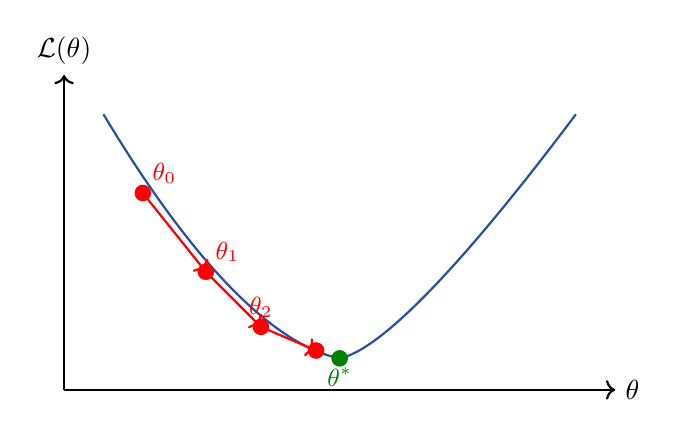
\begin{tikzpicture}[scale=1]
    \draw[->, thick] (0,0) -- (7,0) node[right] {$\theta$};
    \draw[->, thick] (0,0) -- (0,4) node[above] {$\mathcal{L}(\theta)$};

    \draw[thick, circuitblue] (0.5,3.5) .. controls (2,1) and (3,0.5) .. (3.5,0.4) .. controls (4,0.5) and (5,1.5) .. (6.5,3.5);

    \fill[red] (1,2.5) circle (3pt) node[above right, font=\small] {$\theta_0$};
    \draw[->, thick, red] (1,2.5) -- (1.8,1.5);
    \fill[red] (1.8,1.5) circle (3pt) node[above right, font=\small] {$\theta_1$};
    \draw[->, thick, red] (1.8,1.5) -- (2.5,0.8);
    \fill[red] (2.5,0.8) circle (3pt) node[above, font=\small] {$\theta_2$};
    \draw[->, thick, red] (2.5,0.8) -- (3.2,0.5);
    \fill[red] (3.2,0.5) circle (3pt);

    \fill[green!50!black] (3.5,0.4) circle (3pt) node[below, font=\small] {$\theta^*$};
\end{tikzpicture}
\end{center}

\subsection{Variants of Gradient Descent}

\textbf{stochastic gradient descent (SGD)}: instead of computing the gradient over the entire dataset, use a random mini-batch:
\[
\theta_{t+1} = \theta_t - \eta \nabla_\theta \mathcal{L}_{\text{batch}}(\theta_t)
\]
faster per iteration, introduces noise that can help escape local minima.

\textbf{SGD with momentum}: add a ``velocity'' term:
\begin{align}
v_{t+1} &= \beta v_t + \nabla_\theta \mathcal{L}(\theta_t) \\
\theta_{t+1} &= \theta_t - \eta v_{t+1}
\end{align}
smooths out oscillations and accelerates convergence.

\textbf{Adam} (Adaptive Moment Estimation): adapts the learning rate for each parameter based on first and second moments of the gradient:
\begin{align}
m_t &= \beta_1 m_{t-1} + (1-\beta_1) g_t \\
v_t &= \beta_2 v_{t-1} + (1-\beta_2) g_t^2 \\
\theta_{t+1} &= \theta_t - \eta \frac{\hat{m}_t}{\sqrt{\hat{v}_t} + \epsilon}
\end{align}
where $g_t = \nabla_\theta \mathcal{L}(\theta_t)$, $\hat{m}_t = m_t/(1-\beta_1^t)$, $\hat{v}_t = v_t/(1-\beta_2^t)$.

\begin{keypoint}
optimization in QML:
\begin{itemize}
    \item quantum circuit parameters $\theta$ r optimized classically using gradient descent or gradient-free methods
    \item gradients can be computed using the \textbf{parameter shift rule}: $\frac{\partial \langle O \rangle}{\partial \theta_i} = \frac{\langle O \rangle_{\theta_i + \pi/2} - \langle O \rangle_{\theta_i - \pi/2}}{2}$
    \item each gradient evaluation requires running the quantum circuit twice per parameter
    \item total cost for one optimization step: $2p$ circuit evaluations (where $p$ is the number of parameters)
    \item noisy gradients from shot noise and hardware noise make optimization harder
    \item adam and other adaptive methods r commonly used in variational quantum algorithms
\end{itemize}
\end{keypoint}

%% ========================================================
\section{Model Evaluation}
%% ========================================================

\subsection{Train/Test/Validation Split}

\begin{definition}
split ur data into three sets:
\begin{itemize}
    \item \textbf{training set} ($\sim 60$--$80\%$): used to train the model (update parameters)
    \item \textbf{validation set} ($\sim 10$--$20\%$): used to tune hyperparameters (learning rate, circuit depth, etc.) and detect overfitting
    \item \textbf{test set} ($\sim 10$--$20\%$): used only once at the end to estimate generalization performance
\end{itemize}
\end{definition}

\subsection{Cross-Validation}

\begin{definition}
\textbf{k-fold cross-validation}: split data into $k$ folds. train on $k-1$ folds, validate on the remaining fold. repeat $k$ times (each fold serves as validation once). average the $k$ validation scores.
\end{definition}

cross-validation gives a more reliable estimate of generalization performance than a single train/test split, especially with small datasets (common in QML research).

\subsection{Evaluation Metrics for Classification}

\textbf{accuracy}: fraction of correct predictions.
\[
\text{accuracy} = \frac{\text{correct predictions}}{\text{total predictions}}
\]
can be misleading for imbalanced datasets.

\textbf{confusion matrix}: for binary classification:
\[
\begin{pmatrix} \text{TP} & \text{FP} \\ \text{FN} & \text{TN} \end{pmatrix}
\]

\textbf{precision}: of all predicted positives, how many r actually positive?
\[
\text{precision} = \frac{\text{TP}}{\text{TP} + \text{FP}}
\]

\textbf{recall} (sensitivity): of all actual positives, how many did we catch?
\[
\text{recall} = \frac{\text{TP}}{\text{TP} + \text{FN}}
\]

\textbf{F1 score}: harmonic mean of precision and recall.
\[
\text{F1} = 2 \cdot \frac{\text{precision} \cdot \text{recall}}{\text{precision} + \text{recall}}
\]

\textbf{ROC-AUC}: area under the receiver operating characteristic curve. plots true positive rate vs false positive rate at various classification thresholds. AUC $= 1$ is perfect, AUC $= 0.5$ is random guessing.

\begin{example}
suppose a quantum classifier produces:
\begin{itemize}
    \item TP = 45, FP = 5, FN = 10, TN = 40
\end{itemize}

accuracy $= (45 + 40) / 100 = 85\%$

precision $= 45 / (45 + 5) = 90\%$

recall $= 45 / (45 + 10) = 81.8\%$

F1 $= 2 \times 0.9 \times 0.818 / (0.9 + 0.818) = 85.7\%$
\end{example}

\subsection{Evaluation Metrics for Regression}

\textbf{MSE}: mean squared error (already defined).

\textbf{MAE}: mean absolute error $= \frac{1}{N}\sum|f(x_i) - y_i|$.

\textbf{$R^2$ score} (coefficient of determination):
\[
R^2 = 1 - \frac{\sum(y_i - f(x_i))^2}{\sum(y_i - \bar{y})^2}
\]
$R^2 = 1$ is perfect, $R^2 = 0$ means the model predicts the mean, $R^2 < 0$ means worse than predicting the mean.

%% ========================================================
\section{Key Classical ML Models (Preview)}
%% ========================================================

well go deep into SVMs and kernel methods in lecture 8 (bcs they connect directly to quantum kernels). heres a quick overview of the main model families:

\subsection{Linear Models}

\[
f(x) = w^T x + b
\]

\begin{itemize}
    \item linear regression: minimize MSE
    \item logistic regression: $\sigma(w^T x + b)$ for binary classification, minimize cross-entropy
    \item perceptron: simplest neural network unit
\end{itemize}

simple, interpretable, fast. but limited to linearly separable problems.

\subsection{Decision Trees and Ensembles}

\begin{itemize}
    \item decision trees: split the feature space into regions using if/then rules
    \item random forests: ensemble of trees (bootstrap aggregating)
    \item gradient boosting (XGBoost, LightGBM): sequentially build trees that correct previous trees' errors
\end{itemize}

extremely effective for tabular data. often the best choice for structured data even today.

\subsection{Support Vector Machines}

separate data with a maximum-margin hyperplane. use the kernel trick to handle non-linear decision boundaries. deep connection to quantum kernels --- well cover this extensively in lecture 8.

\subsection{Neural Networks}

a simple feedforward neural network (MLP):

\begin{center}
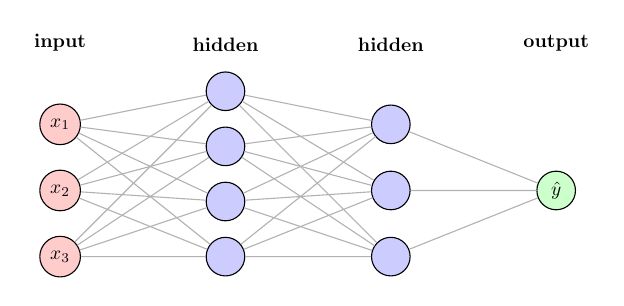
\begin{tikzpicture}[scale=0.7, every node/.style={scale=0.7}]
    % input layer
    \foreach \i in {1,2,3} {
        \node[draw, circle, fill=red!20, minimum size=0.7cm] (i\i) at (0, -\i*1.2) {$x_\i$};
    }
    \node[above] at (0, 0) {\textbf{input}};

    % hidden layer 1
    \foreach \j in {1,2,3,4} {
        \node[draw, circle, fill=blue!20, minimum size=0.7cm] (h\j) at (3, -\j*1.0+0.4) {};
    }
    \node[above] at (3, 0) {\textbf{hidden}};

    % hidden layer 2
    \foreach \k in {1,2,3} {
        \node[draw, circle, fill=blue!20, minimum size=0.7cm] (g\k) at (6, -\k*1.2) {};
    }
    \node[above] at (6, 0) {\textbf{hidden}};

    % output
    \node[draw, circle, fill=green!20, minimum size=0.7cm] (o1) at (9, -2.4) {$\hat{y}$};
    \node[above] at (9, 0) {\textbf{output}};

    % connections
    \foreach \i in {1,2,3} {
        \foreach \j in {1,2,3,4} {
            \draw[gray!60] (i\i) -- (h\j);
        }
    }
    \foreach \j in {1,2,3,4} {
        \foreach \k in {1,2,3} {
            \draw[gray!60] (h\j) -- (g\k);
        }
    }
    \foreach \k in {1,2,3} {
        \draw[gray!60] (g\k) -- (o1);
    }
\end{tikzpicture}
\end{center}

each connection has a weight, each node applies a nonlinear activation function $\sigma$ (ReLU, sigmoid, tanh). the output is:
\[
\hat{y} = \sigma(W_3 \cdot \sigma(W_2 \cdot \sigma(W_1 x + b_1) + b_2) + b_3)
\]

\begin{itemize}
    \item \textbf{MLP}: stacked linear layers with nonlinear activations
    \item \textbf{CNN}: convolutional layers for spatial data (images)
    \item \textbf{RNN/LSTM/Transformer}: sequential/attention-based architectures for sequence data
\end{itemize}

the dominant paradigm in modern ML. quantum neural networks (PQCs) r inspired by classical NNs but have fundamentally diff properties (unitary transformations, entanglement, exponential state space).

\subsection{Kernel Methods}

map data to a high-dimensional feature space and use linear methods there. the kernel trick avoids explicitly computing the feature map. this is the \textbf{direct classical ancestor of quantum kernel methods}.

\begin{keypoint}
the two main paradigms of QML mirror classical ML:
\begin{enumerate}
    \item \textbf{quantum kernel methods}: the quantum computer computes a kernel function $K(x_i, x_j) = |\braket{\phi(x_i)|\phi(x_j)}|^2$ that encodes the data in a quantum feature space. classification/regression is done classically using this kernel.
    \item \textbf{variational quantum models}: analogous to neural networks. parameterized quantum circuits with trainable parameters, optimized end-to-end. the quantum equivalent of ``learn the feature map and the classifier jointly.''
\end{enumerate}
schuld (2021) showed that both paradigms r mathematically equivalent (all variational models can be seen as kernel methods), but they differ in practice (training dynamics, computational cost, generalization).
\end{keypoint}

%% ========================================================
\section{Statistical Learning Theory Basics}
%% ========================================================

\subsection{Generalization}

the central question of ML: if the model does well on training data, will it do well on \textbf{new, unseen} data?

\begin{definition}
the \textbf{generalization error} (true risk) is:
\[
R(\theta) = \mathbb{E}_{(x,y) \sim \mathcal{D}}[\mathcal{L}(f_\theta(x), y)]
\]
where $\mathcal{D}$ is the true data distribution. we cant compute this directly (we dont know $\mathcal{D}$), so we estimate it with the test set.
\end{definition}

\textbf{generalization gap}: $R(\theta) - R_{\text{emp}}(\theta)$ --- the difference between true risk and empirical (training) risk. small gap $=$ good generalization.

\subsection{VC Dimension}

\begin{definition}
the \textbf{VC dimension} of a hypothesis class $\mathcal{H}$ is the largest set of points that $\mathcal{H}$ can shatter (classify correctly for all possible labelings).
\end{definition}

\begin{example}
\begin{itemize}
    \item linear classifiers in $\mathbb{R}^2$: VC dimension = 3 (can shatter any 3 non-collinear points, cant shatter 4 points)
    \item linear classifiers in $\mathbb{R}^d$: VC dimension = $d + 1$
    \item single-layer neural network with $p$ parameters: VC dimension $\sim O(p)$
\end{itemize}
\end{example}

the VC dimension bounds generalization:
\[
R(\theta) \leq R_{\text{emp}}(\theta) + O\left(\sqrt{\frac{d_{\text{VC}} \log(N/d_{\text{VC}})}{N}}\right)
\]

so: if $N \gg d_{\text{VC}}$, the generalization gap is small.

\begin{keypoint}
for QML, caro et al. (2022) proved generalization bounds showing that quantum models with $t$ trainable gates can learn from $O(t)$ training examples. this is favorable --- it means quantum models dont necessarily need huge datasets to generalize, which is important bcs preparing large quantum datasets can be expensive.
\end{keypoint}

%% ========================================================
\section{Dimensionality Reduction}
%% ========================================================

\subsection{Principal Component Analysis (PCA)}

\begin{definition}
\textbf{PCA} finds the directions of maximum variance in the data. project the data onto the top $k$ principal components (eigenvectors of the covariance matrix with the largest eigenvalues).
\end{definition}

\[
\text{covariance matrix: } \Sigma = \frac{1}{N}\sum_{i=1}^N (x_i - \bar{x})(x_i - \bar{x})^T
\]

eigendecompose $\Sigma = V \Lambda V^T$. the first $k$ columns of $V$ define the projection.

\begin{intuition}
PCA has a quantum analogue: \textbf{quantum PCA} uses QPE to extract the eigenvalues of the quantum state's density matrix. this can be exponentially faster than classical PCA for certain input models (the HHL paper connects here). but the input assumptions r strong and debated.
\end{intuition}

%% ========================================================
\section{Summary}
%% ========================================================

\begin{keypoint}
classical ML concepts that carry over directly to QML:
\begin{enumerate}
    \item \textbf{supervised learning}: learn $f: X \to Y$ from labeled data. quantum version: variational quantum classifiers, quantum kernel classifiers.
    \item \textbf{loss functions}: MSE, cross-entropy, hinge. quantum version: expectation values of observables.
    \item \textbf{gradient descent}: iterative parameter updates. quantum version: parameter shift rule for quantum gradients.
    \item \textbf{bias-variance tradeoff}: circuit depth controls model complexity. too shallow = underfitting, too deep = overfitting + noise.
    \item \textbf{regularization}: L2 penalty, dropout, early stopping. quantum version: circuit depth restriction, noise as regularizer.
    \item \textbf{evaluation metrics}: accuracy, precision, recall, F1, AUC --- same metrics used for quantum classifiers.
    \item \textbf{generalization theory}: VC dimension, generalization bounds. quantum version: quantum VC dimension, effective dimension.
    \item \textbf{kernel methods}: the bridge between classical and quantum ML. quantum kernel methods r a direct extension of classical kernel methods.
\end{enumerate}
understanding these classical concepts is essential. QML doesnt replace them --- it extends them.
\end{keypoint}

next: SVMs, kernel methods in depth, and the neural network perspective. this is where the connection to quantum ML becomes explicit.

\end{document}
